% Created 2016-09-22 Thu 14:03
\documentclass[12pt,a4]{article}


\usepackage{hyperref}
\usepackage{minted}
\usepackage{fontspec,xltxtra,xunicode}
\setmainfont[Scale=0.9]{Lato}
\setmonofont[Scale=0.7]{Menlo}
\author{Vittorio Zaccaria}
\date{\today}
\title{Some notes on functionalization of mashup composition}
\hypersetup{
 pdfauthor={Vittorio Zaccaria},
 pdftitle={Some notes on functionalization of mashup composition},
 pdfkeywords={},
 pdfsubject={},
 pdfcreator={Emacs 24.5.1 (Org mode 8.3.6)}, 
 pdflang={English}}
\begin{document}

\maketitle
\tableofcontents


\section{Background}
\label{sec:orgheadline1}

It is well understood that the CDT model allows for a declarative expression of
the type of a context \(c\) which we will broadly assume to be values/parameters
associated with the situational needs in which the query must be answered.

\vspace{0.5cm}
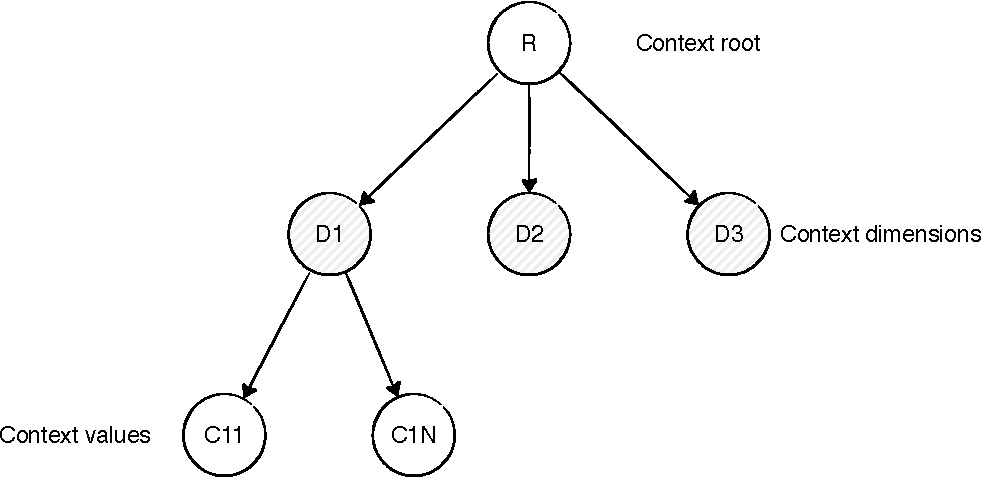
\includegraphics[width=.9\linewidth]{./key/page-1-crop.pdf}
\vspace{0.5cm}

Each dimension \(D_d\) has one value of type indicated by one of children
\(C_{d,i}\), also called \textbf{conceptual nodes}. Each children \(C\) provides a \textbf{view}, i.e.
some way of extracting interesting data from a particular data store (being it a
database or a online service). Effectively, this is a function from the context
\(c\) to a set of actual values of the store. We might see this as the information
value stored into a standard tree leaf.

\begin{minted}[linenos]{haskell}
data Context       = (InterestTopic, Role, Maybe Location, Maybe Interface)
data InterestTopic = Orders (DateRange) | Clients | Food FoodInfo
data View a        = Context -> a

cdt :: Tree (View a)
\end{minted}

The actual view creation can be seen as a \texttt{fold} operation \(\phi\) across the tree, where
the values effectively folded are the views. The fold operation might depend on
the context values as well \[ \phi(c, v_a, v_1) \rightarrow v_a \]
\end{document}